\chapter{Mathematische Theorie}

In diesem Kapitel wird zunächst unter Verwendung vorher eingeführter Sätze und Definitionen die Existenz und eine fundamentale Eigenschaft der Singulärwertzerlegung formal bewiesen.
Anschließend wird an einem konkreten Beispiel die Berechnung durchgeführt und die SVD visualisiert.
Um das Kapitel abzuschließen, erfolgt eine Beschreibung der wichtigsten beiden Arten der Singulärwertzerlegung.
\section{Beweisführung}
Es wird davon ausgegangen, dass der Leser\footnote{Aus Gründen der besseren Lesbarkeit wird das generische Maskulinum verwendet, wobei alle Geschlechter mit eingeschlossen sind.} mit den Grundlagen der linearen Algebra vertraut ist, insbesondere mit Matrizen und ihren Eigenschaften.
Bekannte Definitionen werden nicht erneut aufgeführt, die einzige Ausnahme bildet \zcref{eigvec}, da diese für jegliche Beweisführung und für das Verständnis in diesem Kapitel unerlässlich ist und deswegen eine Auffrischung sinnvoll erscheint.
\begin{definition}\label{eigvec}
    Sei \(n \in \N\) und \(A \in \R^{n \times n}\). Für
    \begin{equation*}
        Av=\lambda v
    \end{equation*}
    heißen die Lösungen \(\R^{n} \ni v \neq 0\) \textit{Eigenvektoren} und die zugehörigen \(\lambda\) \textit{Eigenwerte}.   
\end{definition}
Vorausgesetzte Sätze werden ohne weiteren Beweis verwendet, aber in wichtigen Fällen dennoch vor Verwendung kurz rekapituliert, wie in \zcref{bes} verdeutlicht.
\begin{repitition}[Basisergänzungssatz]\label{bes}
    Sei \(V\) ein beliebiger Vektorraum, \(L \subseteq V\) linear unabhängig und \(E \subseteq V\) ein Erzeugendensystem von \(V\). Dann kann \(L\) durch Elemente aus \(E\) zu einer Basis von \(V\) ergänzt werden.
\end{repitition}
Um die Existenz der Singulärwertzerlegung für beliebige Matrizen zu beweisen, bedarf es der Hilfe eines anderen Satzes, des sogenannten Spektralsatzes.
Dieser hat keine eindeutige Ausführung, sondern beschreibt vielmehr mehrere verwandte Aussagen der Mathematik, wobei sich in dieser Arbeit auf seine Folgerungen für symmetrische Matrizen beschränkt wird.
Es ist ebenfalls wichtig zu betonen, dass der Spektralsatz zwar hier \enquote{nur} für den Beweis der Singulärwertzerlegung verwendet wird, eine Bezeichnung als Hilfssatz jedoch irreführend wäre, da der Satz für sich genommen bereits eine bedeutende Aussage der linearen Algebra und Funktionalanalysis darstellt.
Um den Spektralsatz für symmetrische Matrizen einführen und anschließend beweisen zu können, benötigen wir zunächst \zcref{complex} und \zcref{gram}.
\begin{lemma}\label{complex}
    Sei \(z \in \C\) und \(a,b \in \R\) mit \(z = a + bi\).\ \(z = \overline{z}\) gilt genau dann, wenn \(z \in \R\).     
\end{lemma}
\begin{proof}
    \enquote{\(\Ra\)}\ Durch \(z = \overline{z}\) gilt
    \begin{align*}
        a + bi &= a -bi\\
        \Lra \quad 2bi &= 0.
    \end{align*}
    Da \(i \neq 0\) muss \(b = 0\), womit \(\mathfrak{Im}(z) = 0\). Also ist \(z = \mathfrak{Re}(z) \in \R\).\ \newline
    \enquote{\(\La\)}\ Folgt direkt aus der Definition.  
\end{proof}

\begin{repitition}[Gram-Schmidtsches Orthonormalisierungsverfahren]\label{gram}
    Sei \(V\) ein euklidischer Vektorraum und \(\{u_1,\ldots,u_n\}\) eine Menge von linear unabhängigen Vektoren in \(V\). 
    Dann kann eine Menge \(\{v_1,\ldots,v_n\}\) aus Vektoren in \(V\)  konstruiert werden, sodass \(\{v_1,\ldots,v_n\}\) orthonormal ist und 
    \begin{equation*}
        \symcal{L}\{v_1,\ldots,v_n\} = \symcal{L}\{u_1,\ldots,u_n\}.
    \end{equation*}
\end{repitition}
\begin{theorem}[Spektralsatz]\label{spec}
    Sei \(n \in \N\) und \(A \in \R^{n \times n} \) quadratisch und symmetrisch. 
    Dann gilt:
    \begin{enumerate}[label= (\roman*)]
        \item \(A\) hat reelle Eigenwerte.\label{spec1}
        \item Es existiert eine orthogonale Matrix \(R \in \R^{n \times n}\), sodass \(R^{-1}AR = \Lambda\) diagonal ist.\label{spec2}
    \end{enumerate}
\end{theorem}
\begin{proof}
    Die Behauptungen werden nacheinander bewiesen (vgl.~\cite{proof:SpectralTom}).

    \vspace{5pt}
    \textbf{Zu}~\ref{spec1}: Sei \(\lambda \in \C\) ein Eigenwert von \(A\) mit zugehörigem Eigenvektor \(v \in \C^{n}\). 
    Dann ist mit \zcref{eigvec}
    \begin{align}
        Av &=\lambda v \notag \label{al21}\\
        \Lra \quad A\overline{v} &= \overline{\lambda}\overline{v},
    \end{align}
    da \(A \in \R\) und somit \(A=\overline{A}\) nach \zcref{complex}. 
    Nun gilt zum einen
    \begin{equation}
        {\left(Av\right)}^T \overline{v} = {\left(\lambda v\right)}^{T} \overline{v} = \lambda {v}^{T} \overline{v} \label{eq22}
    \end{equation}
    und zum anderen
    \begin{equation}
        {\left(Av\right)}^T \overline{v} = v^{T}A^{T}\overline{v} \overset{A\text{ sym.}}{=} v^{T}A\overline{v} \overset{\eqref{al21}}{=} v^{T}\overline{\lambda}\overline{v} = \overline{\lambda}v^{T}\overline{v}. \label{eq23}
    \end{equation}
    Mit~\eqref{eq22}\(=\)\eqref{eq23} ergibt sich
    \begin{equation*}
        \lambda v^{T}\overline{v} = \overline{\lambda}v^{T}\overline{v} .
    \end{equation*}
    Da \(v \neq 0\) ist erhalten wir
    \begin{equation*}
        \lambda = \overline{\lambda}.
    \end{equation*}
    Nach \zcref{complex} ist dann \(\lambda \in \R\), wodurch auch \(v \in \R^{n}\) sein muss.\qed
    \vspace{5pt} 

    \textbf{Zu}~\ref{spec2}: Induktion über \(n \in \N\): \\
    \textit{Induktionsanfang}. 
    Für \(n=1\) sind \(A\) und \(R\) Skalare. 
    Setze \(R=1\). 
    Damit ist \(R\) orthogonal, da \(R^{-1}=R^{T}\) und \(\R \ni A = R^{-1}AR\) trivialerweise diagonal. \\
    \textit{Induktionshypothese}. 
    Die Behauptung~\ref{spec2} gelte für festes, beliebiges \(\N \ni n-1\). 
    Es soll gezeigt werden, dass sie dann auch für \(n\) gilt.  \\
    \textit{Induktionsschritt}.  
    Sei \(\lambda_1\) ein beliebiger Eigenwert von \(A\) mit zugehörigem normalisiertem Eigenvektor \(v_1\), also \(\norm{v_1} = 1\).  
    Nach~\ref{spec1} gilt \(\lambda_1 \in \R\) und \(v_1 \in \R^{n}\). 
    Mit dem Basisergänzungssatz (\zcref{bes}) kann \(v_1\) durch Vektoren \(u_2,\ldots,u_n\) zu einer Basis von \(\R^{n}\) ergänzt werden. 
    Nun kann das Gram-Schmidt’sche Orthonormalisierungsverfahren (\zcref{gram}) angewendet werden, wodurch eine orthonormale Basis \(\{v_1,\ldots,v_n\}\) von \(\R^{n}\) konstruiert wird.  
    Der Leser wird daran erinnert, dass orthonormale Vektoren normiert und orthogonal sind.
    Sei 
    \begin{equation*}
        P = 
        \begin{bmatrix}
            \vert & \vert & \vert & \vert\\
            v_1 & v_2 & \cdots & v_n \\
            \vert & \vert & \vert & \vert
        \end{bmatrix} 
        \in \R ^{n \times n}
    \end{equation*} 
    mit \(v_1,\ldots,v_n\) als Spaltenvektoren und setze \(\R^{n \times n} \ni B = P^{-1}AP = P^{T}AP\).

    Das Ziel ist, die Induktionshypothese auf eine symmetrische Untermatrix \(C \in \R^{\left(n-1\right)\times\left(n-1\right)}\) von \(B\) anzuwenden.\\
    \textit{Schritt 1}.
    Dafür wird zunächst die Symmetrie von \(B\) gezeigt:   
    \begin{equation*}
        B^{T} = {\left(P^{T}AP\right)}^{T} = {\left(AP\right)}^{T}P = P^{T}A^{T}P \overset{A\text{ sym.}}{=} P^{T}AP = B.
    \end{equation*} 
    \textit{Schritt 2}.
    Betrachte jetzt die erste Spalte von \(B\). 
    Die erste Spalte einer beliebigen Matrix erhält man durch Multiplikation mit dem kanonischen Einheitsvektor \(\symbf{e}_1\): 
    \begin{align*}
        B\symbf{e}_1 &= P^{T}AP\symbf{e}_1 \\
        &= P^{T}Av_1 & \left(v_1 \text{ ist die erste Spalte von P}\right) \\
        &= P^{T}{\lambda}_1v_1 & \left({\lambda}_1\text{ ist der Eigenwert zu } v_1\right) \\
        &= P^{T}v_1{\lambda}_1 \\
        &= \brows{v_1 \\ v_2 \\ \rowsvdots \\ v_n}v_1{\lambda}_1 \\
        &= 
        \begin{bmatrix}
                \langle v_1,v_1 \rangle \\ \langle v_2,v_1 \rangle \\ \dots \\ \langle v_n,v_1 \rangle
        \end{bmatrix}
        {\lambda}_1 \\
        &=
        \begin{bmatrix}
            1  \\ 0 \\ \vdots \\ 0
        \end{bmatrix}
        {\lambda}_1. & \bigl(\norm{v_1} = 1 \text{ und bel. } v_i,v_j \in \{v_1,\ldots,v_n\} \text{ orthogonal}\bigr)
    \end{align*}
    Mit der Darstellung als Blockmatrix und durch Symmetrie von \(B\) gilt somit 
    \(
    B = 
    \begin{bmatrix}
        {\lambda}_1 & \symbf{0} \\
        \symbf{0} & C
    \end{bmatrix}
    \)
    mit \(C \in \R^{(n-1) \times (n-1)}\) symmetrisch.

    Nach Induktionshypothese gibt es ein orthogonales \(Q \in \R^{(n-1)\times(n-1)}\) mit \(Q^{T}CQ = D\) diagonal. 
    Damit gilt
    \begin{align*}
        P^{T}AP &= B \\
        &= 
        \begin{bmatrix}
            {\lambda}_1 & \symbf{0} \\
            \symbf{0} & C
        \end{bmatrix} \\
        &=
        \begin{bmatrix}
            {\lambda}_1 & \symbf{0} \\
            \symbf{0} & QDQ^{T}
        \end{bmatrix} \\
        &=
        \begin{bmatrix}
            1 & \symbf{0} \\
            \symbf{0} & Q
        \end{bmatrix}
        \begin{bmatrix}
            {\lambda}_1 & \symbf{0} \\
            \symbf{0} & D
        \end{bmatrix}
        \begin{bmatrix}
            1 & \symbf{0} \\
            \symbf{0} & Q^{T}
        \end{bmatrix}.
    \end{align*}
    Also ist
    \begin{equation*}
        \begin{bmatrix}
            1 & \symbf{0} \\
            \symbf{0} & Q^{T}
        \end{bmatrix}
        P^{T}AP
        \begin{bmatrix}
            1 & \symbf{0} \\
            \symbf{0} & Q
        \end{bmatrix}
        =
        \begin{bmatrix}
            {\lambda}_1 & \symbf{0} \\
            \symbf{0} & D
        \end{bmatrix}.
    \end{equation*} 
    Definiere
    \begin{equation*}
        R = P
        \begin{bmatrix}
            1 & \symbf{0} \\
            \symbf{0} & Q
        \end{bmatrix}. 
    \end{equation*}   
    Es gilt
    \begin{equation*}
        R^{T} =
        \begin{bmatrix}
            1 & \symbf{0} \\
            \symbf{0} & Q^{T}
        \end{bmatrix}
        P^{T}
        =
        \begin{bmatrix}
            1 & \symbf{0} \\
            \symbf{0} & Q^{-1}
        \end{bmatrix}
        P^{-1} 
        =
        R^{-1}.
    \end{equation*}
    Dementsprechend ist \(R\) orthogonal und \(R^{-1}AR = R^{T}AR\) = 
    \(
    \begin{bmatrix}
        {\lambda}_1 & \symbf{0} \\
        \symbf{0} & D
    \end{bmatrix}
    =
    \Lambda
    \)  
    diagonal, da \(D\) diagonal ist.              
\end{proof}
\begin{corollary}\label{cor:spec}
    Sei \(n \in \N\) und \(A \in \R^{n \times n}\) quadratisch und symmetrisch. Dann gilt: \\
    Es existiert eine orthogonale Matrix \(R \in \R^{n \times n}\), sodass \(R^{-1}AR = \Lambda\) diagonal ist, wobei die Diagonalwerte von \(\Lambda \in \R^{n \times n}\) die Eigenwerte von \(A\) und die Spalten von \(R\) die normierten Eigenvektoren von \(A\) sind.  
\end{corollary}
\begin{proof}
    Nach dem Spektralsatz (\zcref{spec}) gibt es ein orthogonales 
    \(
    R=
    \big[
    \begin{matrix}
        v_1 \dots v_n
    \end{matrix}
    \big]
    \)
    mit
    \(v_1,\ldots,v_n \in \R^{n}\) 
    und 
    \(\Lambda = \text{diag}(\lambda_1,\ldots,\lambda_n)\), sodass
    \begin{equation*}
        R^{-1}AR = \Lambda.
    \end{equation*}
    Dann ist
    \begin{equation*}
        AR = R\Lambda,
    \end{equation*} 
    oder spaltenweise
    \begin{equation*}
        Av_i = {\lambda}_i v_i, \quad \text{für } i = 1,\ldots,n.
    \end{equation*}
    Da \(R\) orthogonal ist, sind nach Definition die Spaltenvektoren von \(R\), also \(v_1,\ldots,v_n\), orthonormal.
    Für beliebiges \(v_i\) gilt somit \(\norm{v_i} = 1\), wodurch \(v_i \neq 0\) sein muss.
    Mit \zcref{eigvec} sind also \(v_1,\ldots,v_n\) die (normierten) Eigenvektoren von \(A\) mit zugehörigen Eigenwerten \(\lambda_1,\ldots,\lambda_n\).
    
    \textit{Hinweis}. Mithilfe von Zeilen- und Spaltenvertauschungen innerhalb von \(R\) und \(\Lambda\) kann \(\Lambda\) so geordnet werden, dass \(\lambda_1 \geq \lambda_2 \geq \cdots \geq \lambda_n\).
Diese Sortierung wird für den Rest des Kapitels angenommen.
\end{proof}
\begin{remark}
    Durch \zcref{cor:spec} lässt sich direkt die nützliche Aussage treffen, dass bei einer symmetrischen Matrix Eigenvektoren zu verschiedenen Eigenwerten orthogonal zueinander sind. 
\end{remark}
Nun kann mithilfe der vorangegangenen Sätze die Existenz der Singulärwertzerlegung für beliebige reelle Matrizen bewiesen werden.
Der Beweis orientiert sich dabei an~\cite{chenLecture5Singular2020}.

\begin{theorem}[Singulärwertzerlegung]\label{th:svd}
    Sei \(m,n\in\N\) und \(X \in \R^{m \times n}\). \\
    Dann existieren orthogonale Matrizen \(U \in \R^{m \times m}, V \in \R^{n \times n}\) und eine Diagonalmatrix \(\Sigma \in \R^{m \times n}\), sodass
    \begin{equation*}
        X = U \Sigma V^{T}.
    \end{equation*}
\end{theorem}
\begin{proof}
    Sei \(C = X^{T}X \in \R^{n \times n}\) und \(r = \text{rg}(X) \leq \text{min}(m,n)\).
    Dann ist \(C\) symmetrisch und positiv semidefinit (alle Eigenwerte sind positiv oder gleich \num{0} bei symmetrischen Matrizen). 
    Nach \zcref{cor:spec} gibt es ein orthogonales 
    \begin{equation*}
        \symbf{V} =
        \big[
        \begin{matrix}
            v_1 \dots v_n
        \end{matrix}
        \big]
        \in \R^{n \times n}
    \end{equation*}
    und diagonales \(\R^{n \times n} \ni \Lambda = \text{diag}(\lambda_1,\ldots,\lambda_n)\) mit \(\lambda_1 \geq \cdots \geq \lambda_r > 0 = \lambda_{r+1} = \cdots = \lambda_n\), sodass \(C = V \Lambda V^{T}\).    

    \noindent Definiere \(\sigma_i \coloneq \sqrt{\lambda_i}\) für \(i = 1,\ldots,r\) und
    \begin{alignat*}{2}
        &\Sigma_{i,j} &{}={}& 
            \begin{cases}
                \sigma_i, \quad &i=j. \\
                0, \quad &i \neq j.
            \end{cases} \\
        \Lra \quad &\symbf{\Sigma} &{}={}&  
        \begin{bmatrix}
            \text{diag}(\sigma_i,\ldots,\sigma_r) & \symbf{0} \\
            \symbf{0} & \symbf{0}
        \end{bmatrix}
        \in \R^{m \times n}
    \end{alignat*}
    als Blockmatrix.
    Definiere außerdem
    \begin{equation*}
        u_i = \frac{1}{\sigma_i}Xv_i \in \R^{m}, \quad \text{für } 1 \leq i \leq r.
    \end{equation*}
    Dann sind \(u_1,\ldots,u_r\) orthornomal:
    \begin{align*}
        u_i^{T}u_j &= {\left(\frac{1}{\sigma_i}Xv_i\right)}^{T}\left(\frac{1}{\sigma_i}Xv_j\right) \\
        &= \frac{1}{\sigma_i \sigma_j}v_i^{T}\underbrace{X^{\raisebox{0.2ex}{\(\scriptstyle{T}\)}}X}_{=C}v_j \\
        &= \frac{1}{\sigma_i\sigma_j}v_i^{T}(\lambda_j v_j) & \bigl(\lambda_j \text{ ist Eigenwert zu } v_j \bigr) \\
        &= \frac{\sigma_j}{\sigma_i}v_i^{T}v_j & \bigl(\lambda_j = \sigma_j^{2}\bigr) \\
        &=
        \begin{cases}
            1, \quad & i=j. \\
            0, \quad & i \neq j.
        \end{cases} & \bigl(v_i,v_j \text{ orthonormal}\bigr)
    \end{align*}
    Wie bereits im Beweis des Spektralsatzes können \(u_1,\ldots,u_r\) mithilfe des Basisergänzungssatzes (\zcref{bes}) und des Gram-Schmidt-Verfahrens (\zcref{gram}) durch Vektoren \(u_{r+1}\ldots,u_m \in \R^{m}\) zu einer orthonormalen Basis von \(\R^{m}\) ergänzt werden.
    Damit ist 
    \begin{equation*}
        \symbf{U} =
        \big[
        \begin{matrix}
            u_1 \dots u_{r}u_{r+1} \dots u_m
        \end{matrix}
        \big]
        \in \R^{m \times m}
    \end{equation*}
    orthogonal.   
    Es bleibt zu  zeigen, dass \(XV = U\Sigma\) ist, also:
    \begin{equation*}
        X
        \big[
        \begin{matrix}
            v_1 \dots v_{r}v_{r+1} \dots v_n
        \end{matrix}
        \big]
        =
        \big[
        \begin{matrix}
            u_1 \dots u_{r}u_{r+1} \dots u_m
        \end{matrix}
        \big]
        \begin{bmatrix}
            \begin{matrix}
                \sigma_1 &  &  &  \\
                 & \sigma_2 &  & \\
                 &  &  \raisebox{-0.9ex}{\rotatebox{13}{\(\ddots\)}} &  \\
                 &  &  & \sigma_r
            \end{matrix} & \symbf{0} \\
            \symbf{0} & \symbf{0}
        \end{bmatrix}.
    \end{equation*}
    Für \(1 \leq i \leq r\) gilt \(Xv_i = u_i \sigma_i\) nach Konstruktion. \\
    Für \(i > r\) soll gezeigt werden, dass \(Xv_i = 0u_i  = \symbf{0}\) ist. 
    Betrachte dafür
    \begin{equation*}
        X^{T}Xv_i = Cv_i \overset{(*)}{=} 0v_i = \symbf{0}
    \end{equation*}
    {\small\((*)\) \textit{Der zugehörige Eigenwert zum Eigenvektor} \(v_i\) \textit{ist \num{0} für} \(i>r\).} 
    \vspace{5pt}
    \\
    Damit muss wie erwünscht \(Xv_i = \symbf{0}\) gelten, oder \(X^{T} = \symbf{0}\), wodurch ebenfalls \(Xv_i = \symbf{0}\) folgt.       
    Dementsprechend ist \(X = U \Sigma V^{T}\) und die Aussage ist bewiesen. 
\end{proof}
\begin{remark}\leavevmode
    \vspace{-14pt}
    \begin{itemize}
        \item Die Diagonalwerte von \(\Sigma\) heißen \textbf{\underline{Singulärwerte}} von \(X\) und werden meist absteigend sortiert. 
        \item Die Spalten von \(U\) heißen \textbf{\underline{linke Singulärvektoren}} von \(X\).
        \item Die Spalten von \(V\) heißen \textbf{\underline{rechte Singulärvektoren}} von \(X\). 
    \end{itemize}       
\end{remark}
Nachdem der zentrale Beweis dieses Kapitels geführt und die Existenz der Singulärwertzerlegung für beliebige reelle Matrizen gezeigt wurde, wird nun auf eine wichtige Eigenschaft der SVD eingegangen.

Dafür werden zunächst die vier fundamentalen Unterräume zu einer Matrix nach~\cite[185]{strangLineareAlgebra2003} definiert:
\begin{definition}\label{df:four}
    Sei \(A \in \R^{m \times n}\). Definiere folgende Unterräume zu \(A\): 
    \begin{alignat*}{3}
        \text{\textbullet } &\textit{ Spaltenraum: } 
        &&\text{Bild}(A) &{}={}& \{ b \in \R^m \mid \exists x \in \R^n, Ax = b \}. \\
        \text{\textbullet } &\textit{ Zeilenraum: }
        &&\text{Bild}(A^{T}) &{}={}& \{ z \in \R^n \mid \exists y \in \R^m, A^{T}y = z \}.\\
        \text{\textbullet } &\textit{ Kern/Nullraum: }
        &&\text{Kern}(A) &{}={}& \{ x \in \R^n \mid Ax = \symbf{0} \}.\\
        \text{\textbullet } &\textit{ Linkskern: }
        &&\text{Kern}(A^{T}) &{}={}& \{ y \in \R^m \mid A^{T}y = \symbf{0} \}.
    \end{alignat*}
\end{definition}
Die vier Unterräume geben umfangreichen Aufschluss über die Wirkung einer Matrix auf verschiedene Vektoren und stehen dabei in Verbindung mit zahlreichen Themen der linearen Algebra, wie beispielsweise dem Lösen von Gleichungssystemen.

Die Art der Beziehung zwischen der Singulärwertzerlegung und den vier fundamentalen Unterräumen wird in \zcref{cor:svd} zusammengefasst.
Der Beweis wird nach~\cite[S. 214~f.]{johnstonAdvancedLinearMatrix2021} geführt, vor der Beweisführung wird allerdings \zcref{rep:dim} benötigt.
\begin{repitition}[Dimensionssatz]\label{rep:dim}
    Sei \(A \in \R^{m \times n}\). Dann gilt:
    \begin{equation*}
        \text{df}(A) + \text{rg}(A) = n.
    \end{equation*} 
\end{repitition}
\begin{corollary}\label{cor:svd}
    Sei \(m,n\in\N, X \in \R^{m \times n}\)\ und \(r = \textit{rg}(X)\).  \\
    Dann existieren orthogonale Matrizen \(U \in \R^{m \times m}, V \in \R^{n \times n}\) und eine Diagonalmatrix \(\Sigma \in \R^{m \times n}\), sodass
    \begin{equation*}
        X = U \Sigma V^{T}
    \end{equation*}   
    und es gilt:
    \begin{itemize}
        \item Die ersten \(r\) Spalten von \(U\) sind eine Basis des Spaltenraums von \(X\).
        \item Die letzten \(m-r\) Spalten von \(U\) sind eine Basis des Linkskerns von \(X\).
        \item Die ersten \(r\) Spalten von \(V\) sind eine Basis des Zeilenraums von \(X\).
        \item Die letzten \(n - r\) Spalten von \(V\) sind eine Basis des Kerns von \(X\).          
    \end{itemize}
\end{corollary}
\begin{proof}
    Mit der Singulärwertzerlegung (\zcref{th:svd}) erhalten wir orthogonales
    \begin{alignat*}{2}
        &U &{}={}&
        \big[
        \begin{matrix}
            u_1 \dots u_{r}u_{r+1} \dots u_m
        \end{matrix}
        \big]
        \in \R^{m \times m}, \\
        &V &{}={}&
        \big[
        \begin{matrix}
            v_1 \dots v_{r}v_{r+1} \dots v_n
        \end{matrix}
        \big]
        \in \R^{n \times n} \\
        \intertext{und diagonales} 
        &\Sigma &{}={}&
        \begin{bmatrix}
            \text{diag}(\sigma_i,\ldots,\sigma_r) & \symbf{0} \\
            \symbf{0} & \symbf{0}
        \end{bmatrix}
        \in \R^{m \times n},
    \end{alignat*} 
    sodass
    \(
        X = U \Sigma V^{T}
    \).
    Sei nun \(i \in \{1,\ldots,n\}\) und betrachte 
    \begin{equation*}
        Xv_i = U \Sigma V^{T}v_i \overset{(**)}{=} U \Sigma \symbf{e}_i = U \sigma_i \symbf{e}_i = \sigma_i U \symbf{e}_i = \sigma_i u_i.
    \end{equation*}
    {\small\((**)\) \textit{Für} \(i, j \in \{1,\ldots,n\}\) \textit{sind} \(v_i, v_j\) \textit{orthonormal}.} 
    \vspace{5pt}
    \\
    \textbf{Fall 1}: \(1 \leq i \leq r\). \\
    Damit ist \(\sigma_i > 0\) und
    \begin{equation*}
        X \frac{v_i}{\sigma_i} = u_i.
    \end{equation*} 
    Nach \zcref{df:four} sind dann \(u_1,\ldots,u_r \in \text{Bild}(X)\).
    Nun ist \(\text{dim}(\text{Bild}(X)) = \text{rg}(X) = r\) und da \(\symcal{B}_S = \{u_1,\ldots,u_r\}\) genau \(r\) orthonormale Vektoren enthält, bildet \(\symcal{B}_S\) eine Basis vom \(\text{Bild}(X)\), also vom Spaltenraum. 
    \vspace{5pt} \\
    \textbf{Fall 2}: \(i \geq r+1\). \\
    Damit ist \(\sigma_i = 0\) und
    \begin{equation*}
        Xv_i = \symbf{0}.
    \end{equation*}  
    Nach \zcref{df:four} sind dann \(v_{r+1},\ldots,v_n \in \text{Kern}(X)\).
    Durch \zcref{rep:dim} wissen wir, dass \(\text{dim}(\text{Kern}(X)) = \text{df}(X) = n - r\). 
    Mit \(\symcal{B}_K = \{v_{r+1},\ldots,v_n\}\) haben wir \(n-r\) orthonormale Vektoren gegeben, also bildet \(\symcal{B}_K\) eine Basis vom \(\text{Kern}(X)\).
    
    Die Beweise für die Basen des Linkskerns und des Zeilenraums werden analog gezeigt, indem
    \begin{equation*}
        X^{T}u_i = V \Sigma U^{T} u_i
    \end{equation*}
    betrachtet wird.
\end{proof}
Damit ist die Beweisführung dieser Arbeit abgeschlossen und die Berechnung der Singulärwertzerlegung kann an einem Beispiel veranschaulicht und visualisiert werden.
\section{Beispiel und Visualisierung}
\begin{example}\label{ex:svd}
    Sei 
    \begin{equation*}
        A =
        \begin{bmatrix}
            1 & -1 & 3 \\
            3 & \phantom{-}1 & 1
        \end{bmatrix} \in \R^{2 \times 3}.
    \end{equation*}
    Wir wollen nun die SVD dieser Matrix finden.
    Dafür muss der Beweis der Singulärwertzerlegung (\zcref{th:svd}) mithilfe unserer konkreten Werte schrittweise nachvollzogen werden.
    Zuerst wird also
    \begin{equation*}
        A^{T}A = 
        \begin{bmatrix}
            10 & \phantom{-}2 & \phantom{-}6 \\
            2 & \phantom{-}2 & -2 \\
            6 & -2 & \phantom{-}10
        \end{bmatrix} \in \R^{3 \times 3}
    \end{equation*}
    bestimmt. 
    Davon sollen die Eigenwerte mit zugehörigen normierten Eigenvektoren berechnet werden.
    Für die Eigenwerte muss zunächst das charakteristische Polynom 
    \begin{equation*}
        \text{det}(A - \lambda \symbfit{I}) = 0
    \end{equation*}    
    gesetzt und die Lösungen \(\lambda_i\) für \(i =1,2,3\) gefunden werden.
    Auf die genaue Berechnung wird an dieser Stelle verzichtet, das Ergebnis lautet:
    \begin{equation*}
        \lambda_1 = 16, \quad 
        \lambda_2 = 6, \quad
        \lambda_3 = 0.
    \end{equation*}
    Mit \(\sigma_j = \sqrt{\lambda_j}\) für \(j = 1, 2\) (da \(\text{rg}(A)=2\)) erhalten wir
    \begin{equation*}
        \Sigma=
        \begin{bmatrix}
            4 & \phantom{\surd}0 & 0 \\
            0 & \sqrt{6} & 0
        \end{bmatrix} \in \R^{2 \times 3}.
    \end{equation*}
    Durch die Lösungen \(\R^{3} \ni v_i \neq 0\) von
    \begin{equation*}
        (A - \lambda\symbfit{I})v = \symbf{0}
    \end{equation*}
    ergeben sich die normierten Eigenvektoren
    \begin{equation*}
        \renewcommand{\arraystretch}{1.4}
        v_1 =
        \begin{bmatrix}
            \frac{1}{\sqrt{2}} \\
            0 \\
            \frac{1}{\sqrt{2}} \\
        \end{bmatrix}, \quad
        v_2 =
        \begin{bmatrix*}[r]
            -\frac{1}{\sqrt{3}} \\
            -\frac{1}{\sqrt{3}} \\
            \frac{1}{\sqrt{3}} \\
        \end{bmatrix*}, \quad
        v_3 =
        \begin{bmatrix*}[r]
            -\frac{1}{\sqrt{6}} \\
            \frac{2}{\sqrt{6}} \\
            \frac{1}{\sqrt{6}} \\
        \end{bmatrix*}
    \end{equation*} 
    und damit
    \begin{equation*}
        \renewcommand{\arraystretch}{1.3}
        V^{T} =
        \begin{bmatrix}
            \phantom{-}\frac{1}{\sqrt{2}} & \phantom{-}0 & \frac{1}{\sqrt{2}} \\
            -\frac{1}{\sqrt{3}} & -\frac{1}{\sqrt{3}} & \frac{1}{\sqrt{3}} \\
            -\frac{1}{\sqrt{6}} & \phantom{-}\frac{2}{\sqrt{6}} & \frac{1}{\sqrt{6}} \\
        \end{bmatrix} \in \R^{3 \times 3}.
    \end{equation*}
    Es muss also nur noch \(U \in \R^{2 \times 2}\) bestimmt werden, welches spaltenweise durch
    \begin{equation*}
        u_j = \frac{1}{\sigma_j}Xv_j 
    \end{equation*}
    ausgedrückt wird.
    Wir erhalten also
    \begin{equation*}
        u_1 = \frac{1}{4}
        \begin{bmatrix}
            1 & -1 & 3 \\
            3 & \phantom{-}1 & 1
        \end{bmatrix}
        \begingroup
        \renewcommand{\arraystretch}{1.3}
        \begin{bmatrix}
            \frac{1}{\sqrt{2}} \\
            0 \\
            \frac{1}{\sqrt{2}} \\
        \end{bmatrix}
        =
        \begin{bmatrix}
            \frac{1}{\sqrt{2}} \\
            \frac{1}{\sqrt{2}} \\
        \end{bmatrix}
        \endgroup
    \end{equation*}
    und
    \begin{equation*}
        u_2 = \frac{1}{\sqrt{6}}
        \begin{bmatrix}
            1 & -1 & 3 \\
            3 & \phantom{-}1 & 1
        \end{bmatrix}
        \begingroup
        \renewcommand{\arraystretch}{1.3}
        \begin{bmatrix}
            -\frac{1}{\sqrt{3}} \\
            -\frac{1}{\sqrt{3}} \\
            \phantom{-}\frac{1}{\sqrt{3}} \\
        \end{bmatrix}
        =
        \begin{bmatrix}
            \phantom{-}\frac{1}{\sqrt{2}} \\
            -\frac{1}{\sqrt{2}} \\
        \end{bmatrix}
        \endgroup
        .
    \end{equation*}
    Dadurch ist 
    \begin{equation*}
        \renewcommand{\arraystretch}{1.3}
        U =
        \begin{bmatrix}
            \frac{1}{\sqrt{2}} & \phantom{-}\frac{1}{\sqrt{2}} \\
            \frac{1}{\sqrt{2}} & -\frac{1}{\sqrt{2}}
        \end{bmatrix}
    \end{equation*}
    und die Berechnung ist abgeschlossen mit
    \begin{equation*}
        A =
        \begin{bmatrix}
            1 & -1 & 3 \\
            3 & \phantom{-}1 & 1
        \end{bmatrix}
        =
        \begingroup
        \renewcommand{\arraystretch}{1.3}
        \begin{bmatrix}
            \frac{1}{\sqrt{2}} & \phantom{-}\frac{1}{\sqrt{2}} \\
            \frac{1}{\sqrt{2}} & -\frac{1}{\sqrt{2}}
        \end{bmatrix}
        \endgroup
        \begin{bmatrix}
            4 & \phantom{\surd}0 & 0 \\
            0 & \sqrt{6} & 0
        \end{bmatrix}
        \begingroup
        \renewcommand{\arraystretch}{1.3}
        \begin{bmatrix}
            \phantom{-}\frac{1}{\sqrt{2}} & \phantom{-}0 & \frac{1}{\sqrt{2}} \\
            -\frac{1}{\sqrt{3}} & -\frac{1}{\sqrt{3}} & \frac{1}{\sqrt{3}} \\
            -\frac{1}{\sqrt{6}} & \phantom{-}\frac{2}{\sqrt{6}} & \frac{1}{\sqrt{6}} \\
        \end{bmatrix}
        \endgroup
        =
        U \Sigma V^{T}.
    \end{equation*}
\end{example}
Damit genauer verstanden wird, was genau durch die Singulärwertzerlegung geschieht, betrachten wir die Wirkung der Matrix \(A\) aus \zcref{ex:svd} auf einen Vektor \(v \in \R^{3}\), indem wir \(v\) und \(Av\) grafisch darstellen.  
Da dies an einem einzelnen Vektor schwer visualisiert werden kann, multiplizieren wir \(A\) mit allen Punkten auf der Einheitssphäre, also allen 
\begin{equation*}
    v \in 
    \left\{
    \begin{bmatrix}
        \cos(u)\sin(v) \\ \sin(u)\sin(v) \\ \cos(v)
    \end{bmatrix}
    \in \R^{3}
    \mid
    u \in [0, 2\pi], \, v \in [0, \pi]
    \right\}.
\end{equation*}
Das Ergebnis ist in \zcref{fig:sph} dargestellt.  
\begin{figure}[b]
    \centering
    \begin{subfigure}{0.45\textwidth}
        \centering
        %\caption{}\label{fig:spha}
        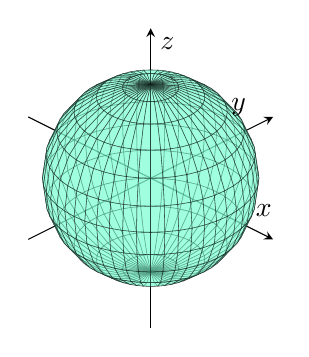
\begin{tikzpicture}
            \begin{axis}[%
                axis equal,
                width=8.5cm,
                height=8.5cm,
                colormap/blackwhite,
                axis lines = center,
                xlabel = {$x$},
                ylabel = {$y$},
                zlabel = {$z$},
                ticks=none, 
                enlargelimits=0.3,
                view/h=45,
                scale uniformly strategy=units only,
            ]
            \addplot3[%
                opacity = 0.5,
                surf,
                line width=0.2pt,
                fill=Aquamarine,
                point meta=100,
                z buffer = sort,
                samples = 25,
                variable = \u,
                variable y = \v,
                domain = 0:180,
                y domain = 0:360,
            ]
            ({cos(u)*sin(v)}, {sin(u)*sin(v)}, {cos(v)});
            \end{axis}
        \end{tikzpicture}
    \end{subfigure}
    \begin{subfigure}{0.45\textwidth}
        \centering
        %\caption{}\label{fig:sphb}
        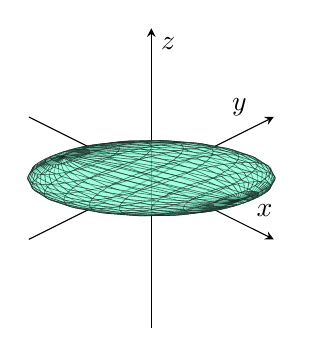
\begin{tikzpicture}
            \begin{axis}[%
                axis equal,
                width=8.5cm,
                height=8.5cm,
                colormap/blackwhite,
                axis lines = center,
                xlabel = {$x$},
                ylabel = {$y$},
                zlabel = {$z$},
                ticks=none, 
                enlargelimits=0.3,
                view/h=45,
                scale uniformly strategy=units only,
                zmin=-0.1,
                zmax=0.1,
                xmin=-3.5,
                xmax=3.5,
                ymin=-3.5,
                ymax=3.5,
                zmin=-3.5, 
                zmax=3.5
            ]
            \addplot3[%
                opacity = 0.5,
                surf,
                line width=0.2pt,
                fill=Aquamarine,
                point meta=100,
                z buffer = sort,
                samples = 25,
                variable = \u,
                variable y = \v,
                domain = 0:180,
                y domain = 0:360,
            ]
            (
                {4/2*cos(u)*sin(v) + 4/2*cos(v) -cos(u)*sin(v) - sin(u)*sin(v) + cos(v) }, 
                {4/2*cos(u)*sin(v) + 4/2*cos(v) +cos(u)*sin(v) +sin(u)*sin(v) -cos(v)}, 
                {0} 
            );
            \end{axis}
        \end{tikzpicture}
    \end{subfigure}
    \caption{Wirkung von \(A\) auf die Einheitssphäre}\label{fig:sph}
  \end{figure}

  Um nachzuvollziehen, wie dieses Ergebnis zustande gekommen ist, verwenden wir die Singulärwertzerlegung und veranschaulichen die Zwischenschritte von \(Av = U \Sigma V^{T}v\) anhand von einzelner Plots (siehe \zcref{fig:svdsph}). 
\begin{figure}[t]
    \centering
    \captionsetup[subfigure]{justification=centering}
    \begin{subfigure}{0.45\textwidth}
        \centering
        \caption{Einheitssphäre}\label{fig:svspha}
        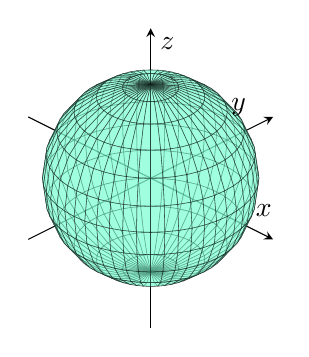
\begin{tikzpicture}
            \begin{axis}[%
                axis equal,
                width=8.5cm,
                height=8.5cm,
                colormap/blackwhite,
                axis lines = center,
                xlabel = {$x$},
                ylabel = {$y$},
                zlabel = {$z$},
                ticks=none, 
                enlargelimits=0.3,
                view/h=45,
                scale uniformly strategy=units only,
            ]
            \addplot3[%
                opacity = 0.5,
                surf,
                line width=0.2pt,
                fill=Aquamarine,
                point meta=100,
                z buffer = sort,
                samples = 25,
                variable = \u,
                variable y = \v,
                domain = 0:180,
                y domain = 0:360,
            ]
            ({cos(u)*sin(v)}, {sin(u)*sin(v)}, {cos(v)});
            \end{axis}
        \end{tikzpicture}
    \end{subfigure}
    \begin{subfigure}{0.45\textwidth}
        \centering
        \caption{Rotation durch \(V^{T}\)}\label{fig:svsphb}
        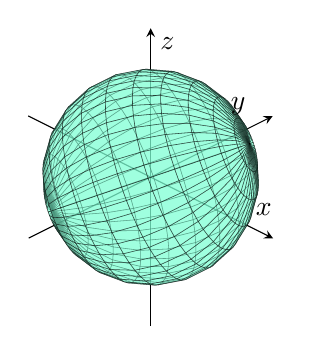
\begin{tikzpicture}
            \begin{axis}[%
                axis equal,
                width=8.5cm,
                colormap/blackwhite,
                height=8.5cm,
                axis lines = center,
                xlabel = {$x$},
                ylabel = {$y$},
                zlabel = {$z$},
                ticks=none,
                enlargelimits=0.3,
                view/h=45,
                scale uniformly strategy=units only,
            ]
            \addplot3[%
                opacity = 0.5,
                surf,
                line width=0.2pt,
                fill=Aquamarine,
                point meta=100,
                z buffer = sort,
                samples = 25,
                variable = \u,
                variable y = \v,
                domain = 0:180,
                y domain = 0:360,
            ]
            (
                {1/sqrt(2)*cos(u)*sin(v) + 0*sin(u)*sin(v) + 1/sqrt(2)*cos(v)}, % x'
                {-1/sqrt(3)*cos(u)*sin(v) - 1/sqrt(3)*sin(u)*sin(v) + 1/sqrt(3)*cos(v)}, % y'
                {-1/sqrt(6)*cos(u)*sin(v) + 2/sqrt(6)*sin(u)*sin(v) + 1/sqrt(6)*cos(v)} % z'
            );
            \end{axis}
        \end{tikzpicture}
    \end{subfigure}
    \begin{subfigure}{0.45\textwidth}
        \centering
        \caption{Skalierung durch \(\Sigma\)}\label{fig:svdsphc}
        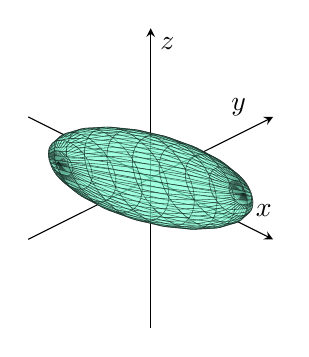
\begin{tikzpicture}
            \begin{axis}[%
                axis equal,
                width=8.5cm,
                colormap/blackwhite,
                height=8.5cm,
                axis lines = center,
                xlabel = {$x$},
                ylabel = {$y$},
                zlabel = {$z$},
                ticks=none,
                enlargelimits=0.3,
                view/h=45,
                scale uniformly strategy=units only,
                xmin=-3.5,
                xmax=3.5,
                ymin=-3.5,
                ymax=3.5,
                zmin=-3.5,
                zmax=3.5
            ]
            \addplot3[%
                opacity = 0.5,
                surf,
                line width=0.2pt,
                fill=Aquamarine,
                point meta=100,
                z buffer = sort,
                samples = 25,
                variable = \u,
                variable y = \v,
                domain = 0:180,
                y domain = 0:360,
            ]
            (
                {4/sqrt(2)*cos(u)*sin(v) + 0*sin(u)*sin(v) + 4/sqrt(2)*cos(v)}, 
                {-sqrt(2)*cos(u)*sin(v) - sqrt(2)*sin(u)*sin(v) + sqrt(2)*cos(v)}, 
                {0} 
            );
            \end{axis}
            \end{tikzpicture}
    \end{subfigure}
    \begin{subfigure}{0.45\textwidth}
        \centering
        \caption{Rotation durch \(U\)}\label{fig:svdsphd}
        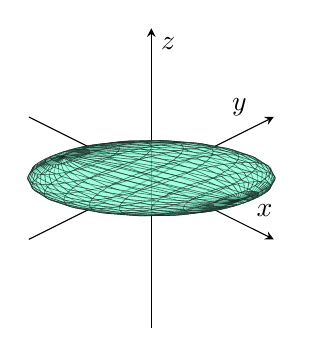
\begin{tikzpicture}
            \begin{axis}[%
                axis equal,
                width=8.5cm,
                height=8.5cm,
                colormap/blackwhite,
                axis lines = center,
                xlabel = {$x$},
                ylabel = {$y$},
                zlabel = {$z$},
                ticks=none, 
                enlargelimits=0.3,
                view/h=45,
                scale uniformly strategy=units only,
                xmin=-3.5,
                xmax=3.5,
                ymin=-3.5,
                ymax=3.5,
                zmin=-3.5, 
                zmax=3.5
            ]
            \addplot3[%
                opacity = 0.5,
                surf,
                line width=0.2pt,
                fill=Aquamarine,
                point meta=100,
                z buffer = sort,
                samples = 25,
                variable = \u,
                variable y = \v,
                domain = 0:180,
                y domain = 0:360,
            ]
            (
                {4/2*cos(u)*sin(v) + 4/2*cos(v) -cos(u)*sin(v) - sin(u)*sin(v) + cos(v) }, 
                {4/2*cos(u)*sin(v) + 4/2*cos(v) +cos(u)*sin(v) +sin(u)*sin(v) -cos(v)}, 
                {0} 
            );
            \end{axis}
        \end{tikzpicture}
    \end{subfigure}
    \caption{Visualisierung der Singulärwertzerlegung}\label{fig:svdsph}
\end{figure}

Grundlage für diese Visualisierung ist das Wissen, dass im euklidischen Raum orthogonale Matrizen Drehungen und Diagonalmatrizen Skalierungen (entlang der Hauptachsen) darstellen.
An dieser Stelle ist auch wichtig zu erwähnen, dass in \zcref{fig:svdsphc} und \zcref{fig:svdsphd} der zu beobachtende Wertebereich vergrößert wurde, also eine größere Streckung durch \(\Sigma\) erfolgt ist, als auf dem Plot zu sehen ist.
Außerdem sei angemerkt, dass ab \zcref{fig:svdsphc} die Darstellung der \(z\)-Achse überflüssig und eigentlich nicht zu empfehlen ist, da sich dort durch die Dimensionsreduktion mittels \(\Sigma\) im zweidimensionalen Raum bewegt wird.
Um eine Vergleichbarkeit der Plots zu verbessern, wird die Darstellung dennoch beibehalten.  

Zusammenfassend zerlegt also die Singulärwertzerlegung eine Matrix in grundlegende geometrische Transformationen: Drehung, Skalierung und gegebenenfalls Dimensionsreduktion oder -erhöhung.

Mit dieser Erkenntnis wird sich dem letzten Abschnitt des theoretischen Teils zugewandt, in dem die wichtigsten beiden Arten der SVD definiert werden.

\section{Arten der Singulärwertzerlegung}

Die Singulärwertzerlegung, die im vorherigen Teil der Arbeit beschrieben wurde, ist die klassische und vollständige Zerlegung.
In den tatsächlichen Anwendungsgebieten, welche im nächsten Kapitel ausgeführt werden, finden häufig Variationen Verwendung.
\begin{definition}\label{df:redsvd}
    Sei \(m,n \in \N,\ A \in \R^{m \times n},\ \text{rg}(A)=r\) und \(A=U \Sigma V^{T}\) die vollständige SVD von \(A\) mit \(U \in R^{m \times m},\ \Sigma \in \R^{m \times n}\) und \(V \in \R^{n \times n}\). \\
    Definiere die \textit{reduzierte SVD} von \(A\):
    \begin{equation*}
        A = U_r \Sigma_r V^{T}_r
    \end{equation*}
    mit
    \begin{alignat*}{2}
        &U_r &{}={}&
        \big[
        \begin{matrix}
            u_1 \dots u_{r}
        \end{matrix}
        \big]
        \in \R^{m \times r}, \\
        &\Sigma_r &{}={}&
        \text{diag}(\sigma_i,\ldots,\sigma_r)
        \in \R^{r \times r}, \\
        &V_r &{}={}&
        \big[
        \begin{matrix}
            v_1 \dots v_{r}
        \end{matrix}
        \big]
        \in \R^{n \times r}.
    \end{alignat*}
\end{definition}
Die in \zcref{df:redsvd} beschriebene Art der Singulärwertzerlegung besitzt den Vorteil, dass eine exakte Berechnung mit deutlich weniger Speicherbedarf möglich ist, insbesondere bei großen Matrizen \(X \in \R^{m \times n}\) mit \(\text{rg}(X) \ll \text{min}(m,n)\). 

Nachteilig ist, dass die Basen für den Kern und Linkskern \enquote{verloren gehen} (siehe \zcref{df:four}), dies spielt für die meisten Anwendungen allerdings eine untergeordnete Rolle.

Bevor zur nächsten Variation übergegangen werden kann, betrachten wir eine weitere Darstellungsform von \zcref{df:redsvd}.
\begin{remark}\label{rem:onesvd}
    Sei
    \begin{equation*}
        A = 
        \big[
            \begin{matrix}
                u_1 \dots u_{r}
            \end{matrix}
        \big]
        \begin{bmatrix}
            \sigma_1 &  & \\
              &  \rotatebox{12}{\(\ddots\)} &  \\
              &  &  \sigma_r \\
        \end{bmatrix}
        \begin{bmatrix}
            v^{T}_1 \\
            \vdots \\
            v^{T}_r \\
        \end{bmatrix}
    \end{equation*}
    wie in \zcref{df:redsvd}. \\
    Dann ist \(A_{1,1} = u_{1,1} \sigma_1 v^{T}_{1,1} + u_{2,1} \sigma_2 v^{T}_{2,1} +\ \cdots \ + u_{r,1} \sigma_r v^{T}_{r,1} \). \\
    Für die andere Komponenten von \(A\) kann die Summe analog gebildet werden. 
    Wir erhalten also
    \begin{alignat*}{2}
        &A_{i,j} &{}={}& \sum_{k=1}^{r} \sigma_k u_{k,i} v^{T}_{k,j}  \\
        \Lra \quad &A &{}={}& \sum_{i=1}^{r} \sigma_i u_i v^{T}_i.
    \end{alignat*}
    Damit kann \(A\) als \textit{Summe von Rang-\num{1}-Matrizen} dargestellt werden, da für \(i \in \{1,\ldots,r\}\) die Zeilen von \((\sigma_i u_i v^{T}_i)\in \R^{m \times n}\) ein Vielfaches von \(v^{T}_i\) und die Spalten ein Vielfaches von \(u_i\) sind. \\
    Beachte, dass \(\sigma_1 \geq \sigma_2 \geq \cdots \geq \sigma_r\) und \(\norm{u_i}=1=\norm{v_i}\), also gilt komponentenweise: \(\sigma_1 u_1 v^{T}_1 \geq \sigma_2 u_2 v^{T}_2 \geq \cdots \geq \sigma_r u_r v^{T}_r\). 
\end{remark}
Nun wird die womöglich interessanteste Art der Singulärwertzerlegung für diverse Anwendungsfälle definiert.
\begin{definition}\label{df:trunsvd}
    Sei \(m,n \in \N,\ A \in \R^{m \times n},\ \text{rg}(A)=r\) und \(A=U_r \Sigma_r V^{T}_r = \sum_{i=1}^{r} \sigma_i u_i v^{T}_i\) die reduzierte SVD von \(A\) mit \(U_r \in R^{m \times r},\ \Sigma_r \in \R^{r \times r}\) und \(V_r \in \R^{n \times r}\). \\
    Für \(k \leq r\) sei die \textit{trunkierte SVD} definiert mit:
    \begin{equation*}
        A \approx \sum_{i=1}^{k} \sigma_i u_i v^{T}_i.
    \end{equation*}
\end{definition}
Zur \zcref{df:trunsvd} sei angemerkt, dass die Approximation von \(A\) für größere Werte von \(k\) zunehmend präziser wird, aber da komponentenweise \(\sigma_1 u_1 v^{T}_1 \geq \cdots \geq \sigma_r u_r v^{T}_r\) gilt (siehe \zcref{rem:onesvd}), kann bereits mit \(k \ll r\) eine gute Annäherung erzielt werden. 

Mit den beiden, in diesem Abschnitt eingeführten, Variationen der Singulärwertzerlegung sind alle wesentlichen Grundlagen für die Vertiefung verschiedener Anwendungsmöglichkeiten der SVD gelegt.
Damit wird der theoretische Teil dieser Arbeit beendet und zum Anwendungsteil übergegangen.